\chapter{Testes de performance}
\label{ch:performance}

Nessa seção vamos comparar o desempenho da busca em profundidade implementada
em Rust com uma versão tradicional implementada em C++, usando
bibliotecas \textit{benchmarking} escritas em Rust. O
objetivo é mostrar que apesar do alto nível de abstração e
flexibilidade da nossa implementação, o desempenho ainda fica próximo
de versões tradicionais do algoritmo que não tem a mesma
flexibilidade, implementadas em C++.

\section{Metodologia}

Os testes realizados vivem sob duas principais categorias,
\textit{Micro Benchmarking} de alta precisão e \textit{Micro
Benchmarking} estatístico. Micro
benchmarking de alta precisão executa apenas uma vez pedaço de código
e mensura estatísticas como, quantidade de
instruções realizadas pelo processador, acesso ao cache e uso de RAM.
Enquanto, o micro benchmarking estatístico, se refere a múltiplas
execuções de um pedaço de código, onde é realizada a coletas de várias
amostras, nesse tipo de teste, é mensurado medidas de tendência
central e dispersão, como a média e desvio padrão do tempo de execução.
Para facilitar a realização desses testes e a coleta de dados, importamos duas
bibliotecas públicas escritas em Rust, \cite{criterionrust} e
\cite{gungraunrust} para o Micro Benchmark estatístico e Micro
Benchmark de alta precisão respectivamente.

Para viabilizar a coleta de dados de funções em C++ usando as
bibliotecas implementadas em Rust, foi necessário criar uma FFI
(Foreign Function Interface) para permitir que código C++ interaja
com o código das bibliotecas em Rust. Essa implementação, se deu
especificando um bloco \texttt{extern "C"} para permitir que as
funções sejam identificadas unicamente pelo seu nome, por exemplo:

\begin{lstlisting}[language=C++, caption={Exemplo de interface FFI escrita em C++}, label=list:externCFfi]
extern "C" {
void* mk_adjacency_list(size_t node_amt) { ... }

void add_edge_unchecked(void* graph, size_t n, size_t m) { ... }

void dfs(void* graph, size_t start) { ... }
}
\end{lstlisting}

Feito isso, fomos capazes de importar e usar essa interface em código
Rust e implementar um encapsulador:

\begin{lstlisting}[language=Rust, caption={Exemplo de uso de interface FFI escrita em Rust}, label=list:externCFfi]
unsafe extern "C" {
    fn mk_adjacency_list(node_amt: usize) -> *mut std::ffi::c_void;
    fn add_edge_unchecked(graph: *mut std::ffi::c_void, n: usize, m: usize);
    fn dfs(graph: *mut std::ffi::c_void, start: usize);
}

pub struct AdjacencyListCpp {
    ptr: *mut std::ffi::c_void,
}

impl AdjacencyListCpp {
    pub fn new(node_amt: usize) -> Self { ... }

    pub fn add_edge_unchecked(&self, n: usize, m: usize) { ... }

    pub fn dfs(&self, start: usize) { ... }
}
\end{lstlisting}

Exemplos completos de código são acessíveis no
caminho~\url{https://github.com/mpazmarcato/Trabalho-U1-Grafos/tree/main/crates/cpp-api}.

\subsection{Micro Benchmarking estatístico}

O processo de Micro Benchmarking implementado pela
biblioteca~\cite{criterionrust} funciona em quatro etapas,
Aquecimento, Medição, Análise e Comparação com o resultado
anterior~\citep{bheislerAnalysisProcess}.
Entretanto, não levaremos em conta o resultado da última etapa. A
primeira etapa serve para aquecer o cache da CPU, de forma que seja
reduzida a quantidade de casos atípicos na
amostra~\citep{bheislerAnalysisProcess}. A segunda etapa
realiza a medição dos tempos de execução e a terceira etapa realiza o
cálculo de estatísticas como média, moda e mediana dos dados medidos.

A biblioteca também gera gráficos automaticamente usando o
programa~\href{http://gnuplot.info/}{Gnuplot}. A biblioteca também argumenta
que as amostras de bom benchmark deve formam uma linha de regressão
quando plotadas num gráfico~\citep{bheislerAnalysisProcess}.

\subsection{Micro Benchmarking de alta precisão}

O processo de Micro Benchmarking implementado pela
biblioteca~\cite{gungraunrust}, funciona de uma maneira bastante
diferente do Criterion, este executa um trecho de código apenas uma
vez e coleta as estatísticas usando o
\href{https://valgrind.org/}{Valgrind}. Estas estatísticas incluem
quantidade estimada de ciclos da CPU, quantidade de instruções
realizadas, quantos acertos de cache L1 e L2 e outros. O processo de
configuração e uso é praticamente idêntico ao do Criterion.

\section{Implementação dos testes}

Vamos realizar testes apenas para a Busca em
profundidade. Todos os testes serão realizados numa lista de
adjacência em grafos completos, ou seja, que há arestas entre todos
os nós. Essa escolha advém da ideia de que queremos maximizar o uso
de recursos e quantidade de instruções, possivelmente evidenciando
as diferenças que favorecem a implementação em C++.

Como não foi apresentada anteriormente, aqui está a implementação da
busca em profundidade em C++. Definimos uma classe para a lista de
adjacência em C++ e realizamos a implementação tradicional da busca,
tomando o cuidado para pré-alocar a pilha e o dicionário de
visitados, assim como a implementação em Rust e para evitar alocações
no meio da busca.

\begin{lstlisting}[language=C++, caption={Implementação da busca em profundidade em C++}]
class AdjacencyList {
   private:
    std::vector<std::vector<size_t>> data;

   public:
    AdjacencyList(size_t node_amt) : data(node_amt) {}

    size_t order() { return data.size(); }

    std::vector<size_t>& neighbors(const size_t node) {
        static std::vector<size_t> empty;
        return (node < order()) ? data[node] : empty;
    }

    void dfs(const size_t start) {
        std::vector<size_t> stack;
        std::unordered_set<size_t> visited;

        stack.reserve(order());
        visited.reserve(order());

        stack.push_back(start);
        visited.insert(start);

        while (!stack.empty()) {
            const auto current = stack.back();
            stack.pop_back();

            for (const auto& neighbor : neighbors(current)) {
                if (visited.insert(neighbor).second) {
                    stack.push_back(neighbor);
                }
            }
        }
    }
};
\end{lstlisting}

O código fonte da geração do grafo e da
criação dos testes é a seguinte:

\begin{lstlisting}[language=Rust, caption={Código fonte da geração do grafo completo}]
pub fn create_complete_graph(size: usize) -> AdjacencyMatrix {
    let mut matrix = vec![vec![0; size]; size];
    for (i, row) in matrix.iter_mut().enumerate() {
        for (j, val) in row.iter_mut().enumerate() {
            if i != j {
                *val = 1;
            }
        }
    }
    AdjacencyMatrix(matrix)
}
\end{lstlisting}

\subsection{Micro Benchmarking estatístico}

Realizamos 3 testes performando a busca num grafo completo, os testes
se diferenciam pela ordem do grafo gerado. Foram gerados grafos com
500 nós, 1000 e 2000 nós.

\begin{lstlisting}[language=Rust, label={code:micro-dfs}, caption={Código fonte dos testes de Micro Benchmark estatístico da DFS.}]
fn bench_dfs_comparison(c: &mut Criterion) {
    let sizes = vec![500, 1000, 2000];

    let mut group = c.benchmark_group("dfs");

    for size in sizes {
        let g = create_complete_graph(size);
        let rust_list = AdjacencyList::from_adjacency_matrix(&g);
        let cpp_list = AdjacencyListCpp::from_adjacency_matrix(&g);

        group.bench_with_input(
            BenchmarkId::new("rust", size),
            &size,
            |b, _| b.iter(|| rust_list.dfs(0).for_each(|_| ()))
        );

        group.bench_with_input(
            BenchmarkId::new("cpp", size),
            &size,
            |b, _| b.iter(|| cpp_list.dfs(0))
        );
    }

    group.finish();
}

criterion_group! {
    name = benches;
    config = Criterion::default()
        .measurement_time(std::time::Duration::from_secs(30));
    targets = bench_dfs_comparison
}

criterion_main!(benches);
\end{lstlisting}

\subsection{Micro Benchmarking de alta precisão}

No Micro Benchmark de alta precisão, foi realizado apenas um teste da busca em
profundidade para um grafo completo com 1000 nós. É importante
ressaltar que a parte do código que é responsável pela inicialização
do grafo também é mensurada no teste, pois é uma limitação da biblioteca.
O código que implementa o Micro Benchmark é o seguinte:

\begin{lstlisting}[language=Rust, label={code:microhp-dfs}, caption={Código dos testes de Micro Benchmark de alta precisão da implementação da DFS.}]
fn setup() -> AdjacencyList {
    AdjacencyList::from_adjacency_matrix(&create_complete_graph(1000))
}

fn cpp_setup() -> AdjacencyListCpp {
    AdjacencyListCpp::from_adjacency_matrix(&create_complete_graph(1000))
}

#[library_benchmark]
fn single_shot_dfs() {
    setup().dfs(black_box(0)).for_each(|_| ())
}

#[library_benchmark]
fn single_shot_cpp_dfs() {
    cpp_setup().dfs(black_box(0))
}

library_benchmark_group! {
    name = bench_dfs_group;
    benchmarks = single_shot_dfs, single_shot_cpp_dfs
}

main!(library_benchmark_groups = bench_dfs_group);
\end{lstlisting}

Na código~\ref{code:microhp-dfs}, Note o uso da função \texttt{black\_box} na
chamada das duas buscas (linhas 11 e 16), ela serve para que o
compilador não pré-calcule a computação realizada pela DFS.

O mesmo não precisa no Micro Benchmark estatístico pois o tipo da variável
\texttt{group} na código~\ref{code:micro-dfs} já garante isso automaticamente.

\section{Resultados}

\subsection{Especificações da máquina usada nos testes}

Para realizar os testes, usamos um computador com as seguintes
configurações:

\begin{table}[!ht]
  \centering
  \caption{Especificações do sistema de teste}
  \begin{tabular}{llll}
    \toprule
    \multirow{3}{3cm}{Hardware}
    & Processador & AMD Ryzen 9 5900XT          & \\
    & GPU         & Nvidia Geforce RTX 4060 Ti  &    \\
    & RAM         & 32GB RAM                    & \\
    & &   &    \\
    \multirow{6}{3cm}{Software}
    & Sistema Operacional & Arch Linux x86\_64        &    \\
    & Kernel              & Linux 6.17.1-arch-1-1     &    \\
    & Compilador Rust     & rustc 1.90.0 (2025-09-14) &    \\
    & Versão do Cargo     & 1.90.0 (2025-07-30)       &    \\
    & Compilador C++      & clang 20.1.8              &    \\
    & Versão do Valgrind  & 3.25.1                    &    \\
    & &   &    \\
    \bottomrule
  \end{tabular}
\end{table}

\subsection{Busca em profundidade}

\subsubsection{Micro Benchmark estatístico}

Começaremos pelos testes de Micro Benchmarking estatístico, que exibem
estatísticas sobre o tempo de execução dos algoritmos coletadas de
várias iterações, ou amostras. Como as proporções das versões de um
grafo com 500, 1000 e 2000 nós foram parecidas, nesse texto
exibiremos apenas o resultado do benchmark de um grafo com 500 nós.
Portanto, tivemos:

\begin{figure}[!ht]
  \centering
  \caption{Gráfico de inclinação do Micro Benchmark estatístico da DFS em Rust.}
  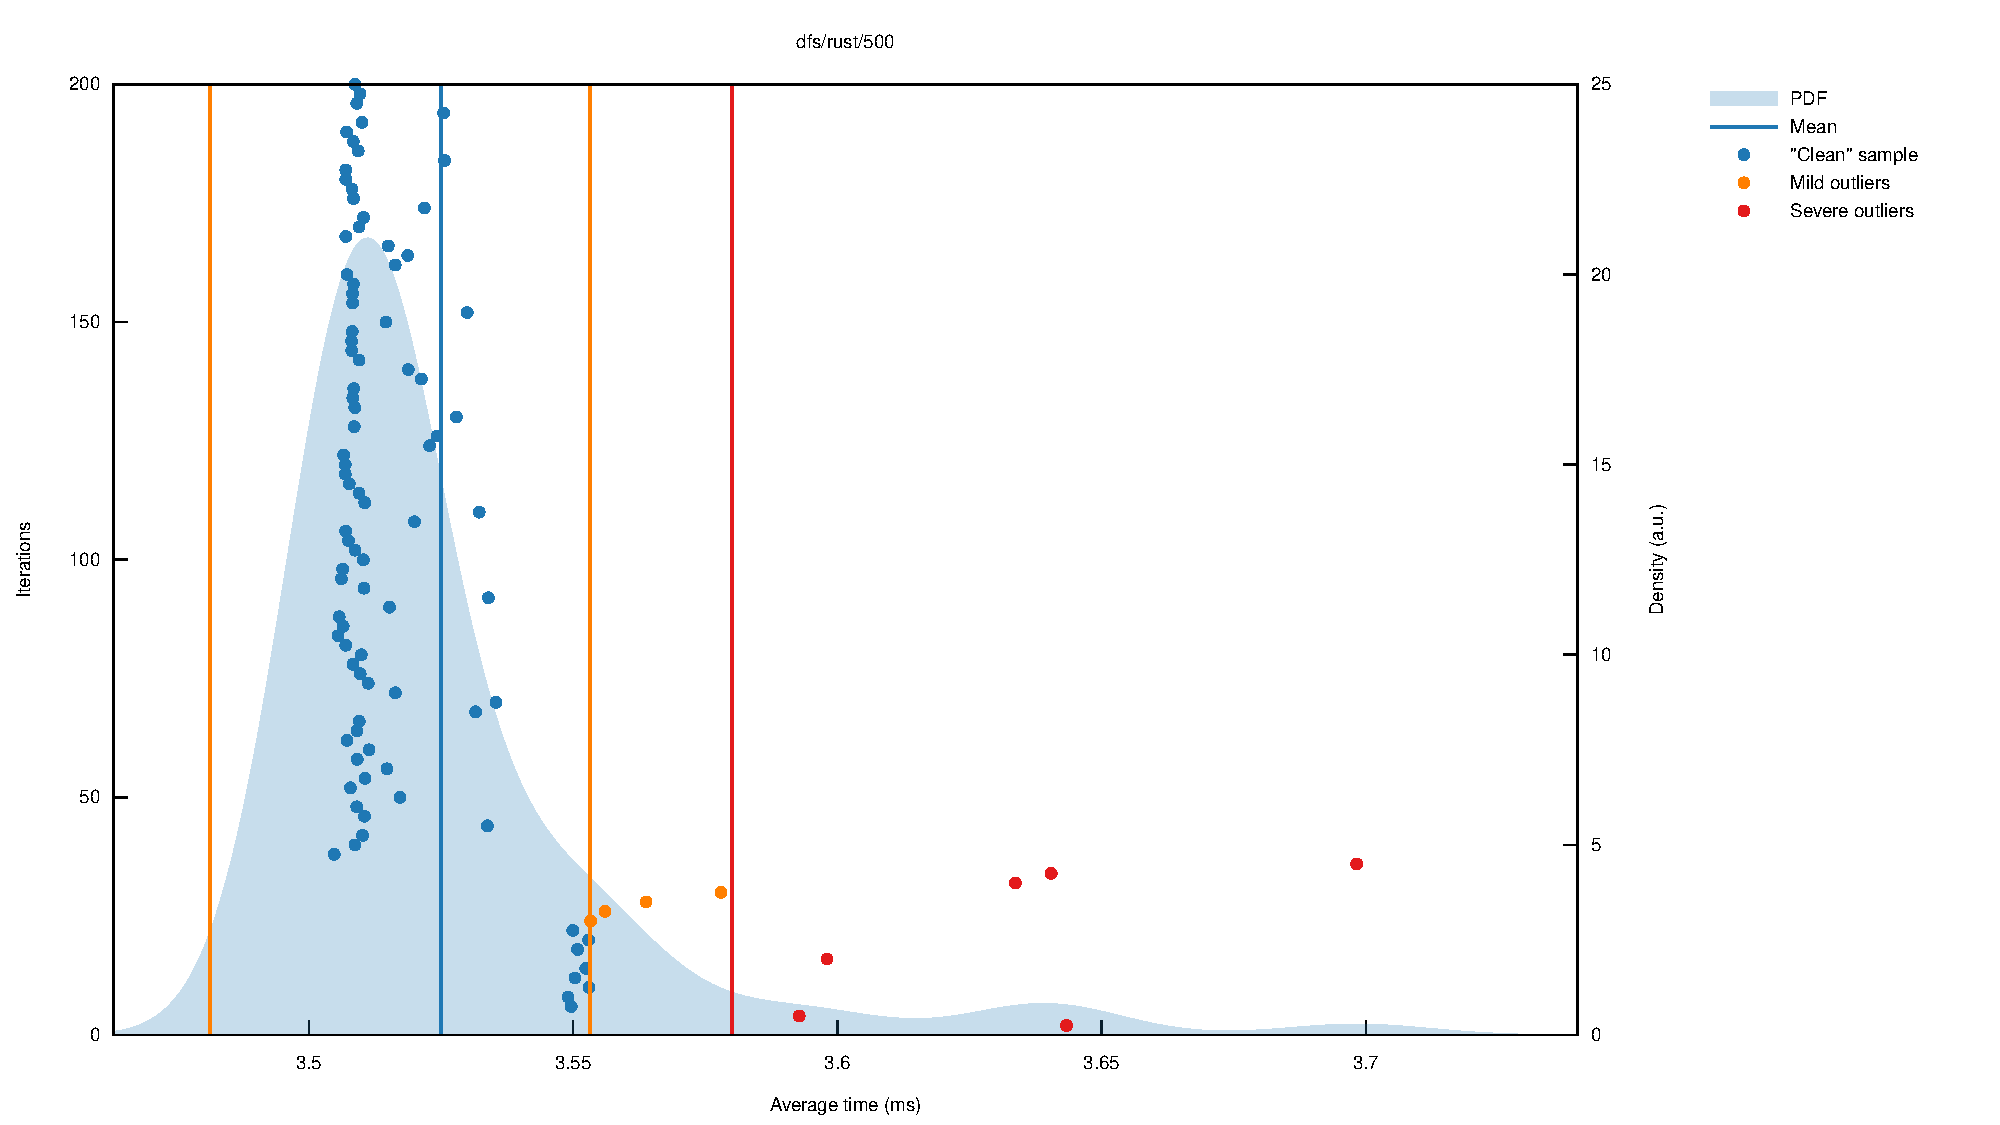
\includegraphics[width=\textwidth]{figures/rust-dfs-500.pdf}
  \label{graph:rust-dfs-slope}
\end{figure}
\FloatBarrier

Na figura~\ref{graph:rust-dfs-slope}, os pontos azuis são amostras
"limpas", os pontos vermelhos representam casos atípicos sevéros, os
pontos amarelos representam casos atípicos médios, seguindo o método de
Tukey~\citep{criterionrust}, as retas amarelas e vermelhas
representam as cotas superiores e inferiores dessas medidas. O fundo
azul representa a função de probabilidade desse teste e a reta azul
representa a média, nesse caso, em torno de 3.54 ms.

Para validar se o benchmark foi bom, analisemos a reta de regressão
das amostras desse teste:

\begin{figure}[!ht]
  \centering
  \caption{Gráfico de regressão das amostras do Micro Benchmark
  estatístico da DFS em Rust.}
  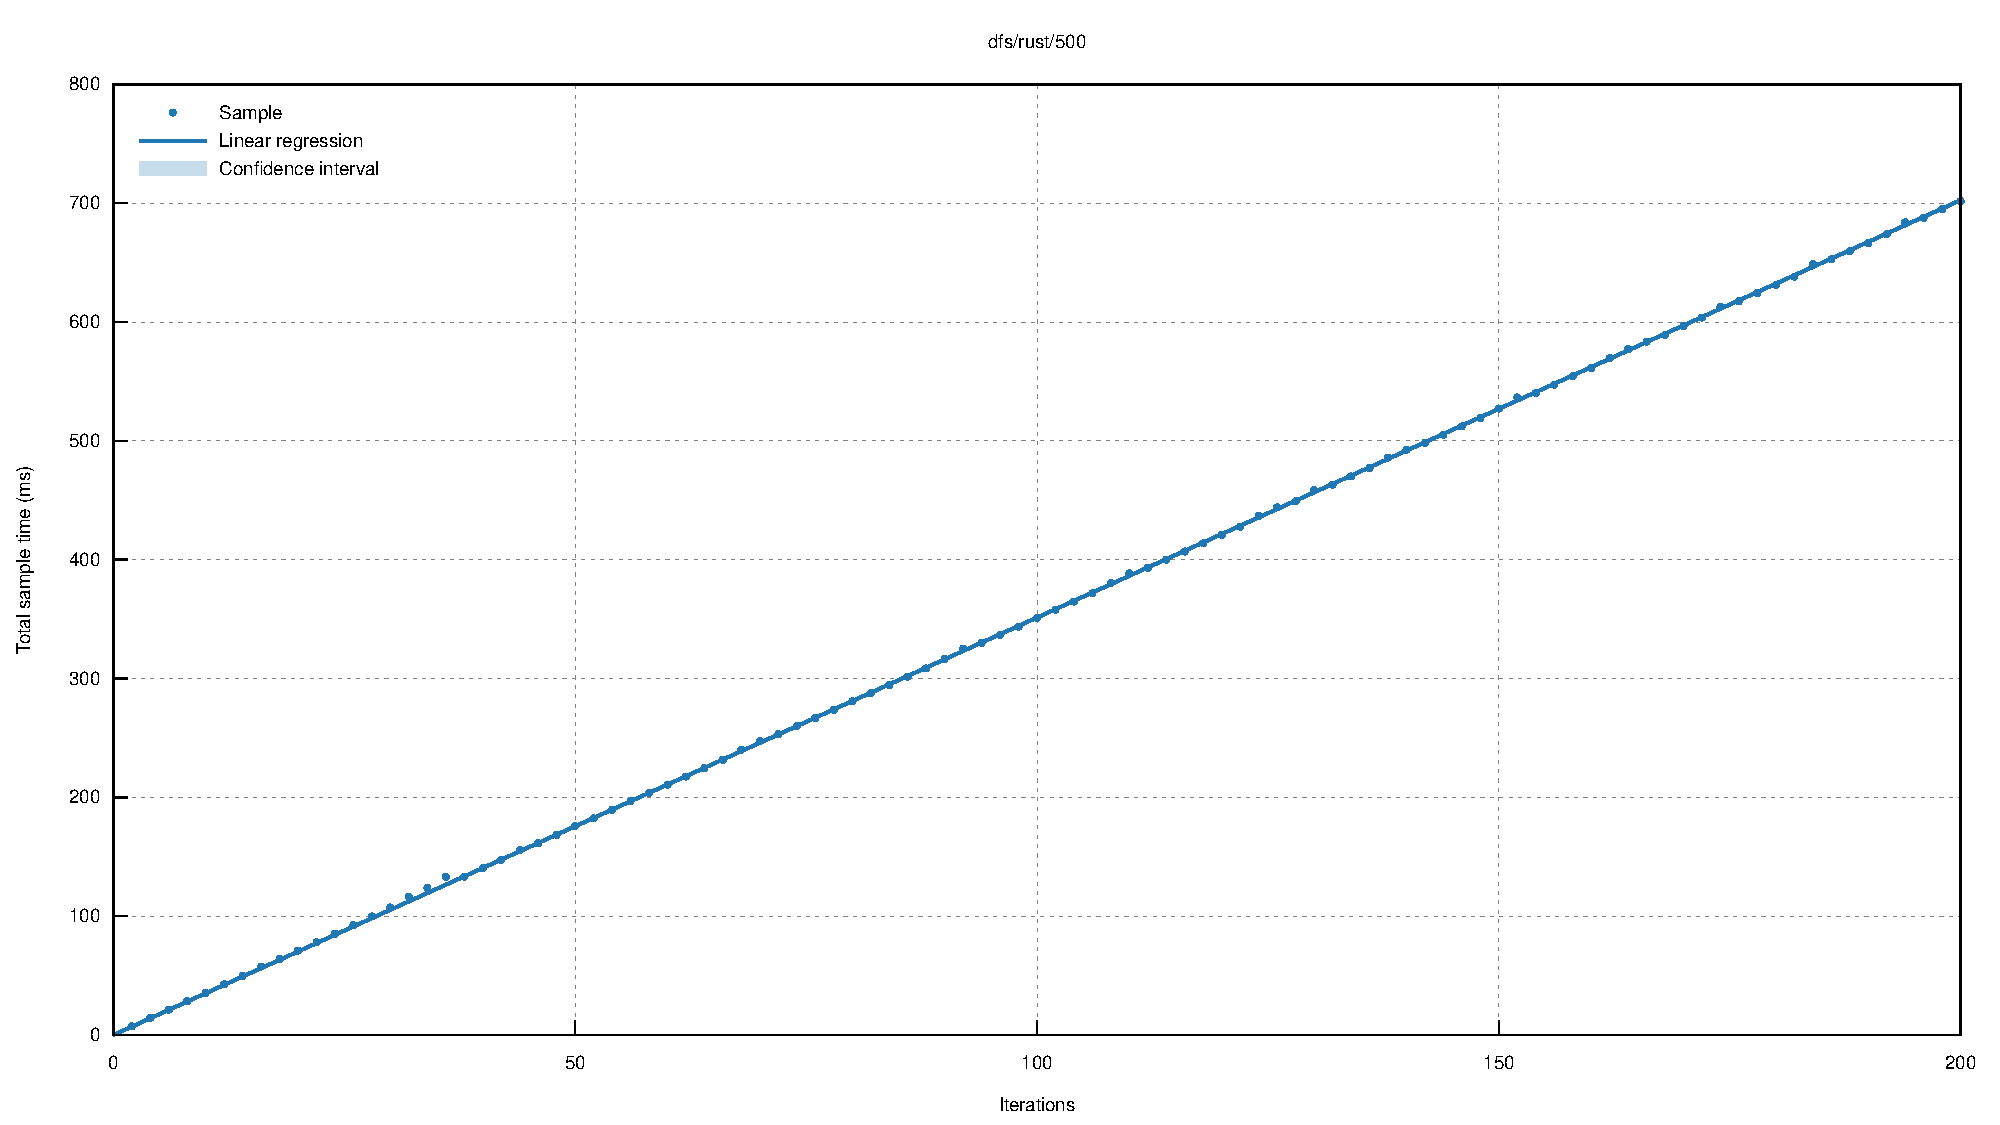
\includegraphics[width=\textwidth]{figures/rust-dfs-500-regression.pdf}
  \label{graph:rust-dfs-regression}
\end{figure}
\FloatBarrier

Na figura~\ref{graph:rust-dfs-regression}, os pontos azuis
representam as amostras coletadas e a linha azul representa a reta de
regressão sobre as amostras. Se o teste produz uma reta de regressão
que grosseiramente passa por todas as amostras, o teste é considerado
um bom benchmark~\citep{criterionrust}, o que nesse caso é verdade.

Quanto aos teste realizado na implementação em C++, obtivemos o seguinte:

\begin{figure}[!ht]
  \centering
  \caption{Gráfico de inclinação do Micro Benchmark estatístico da DFS em C++.}
  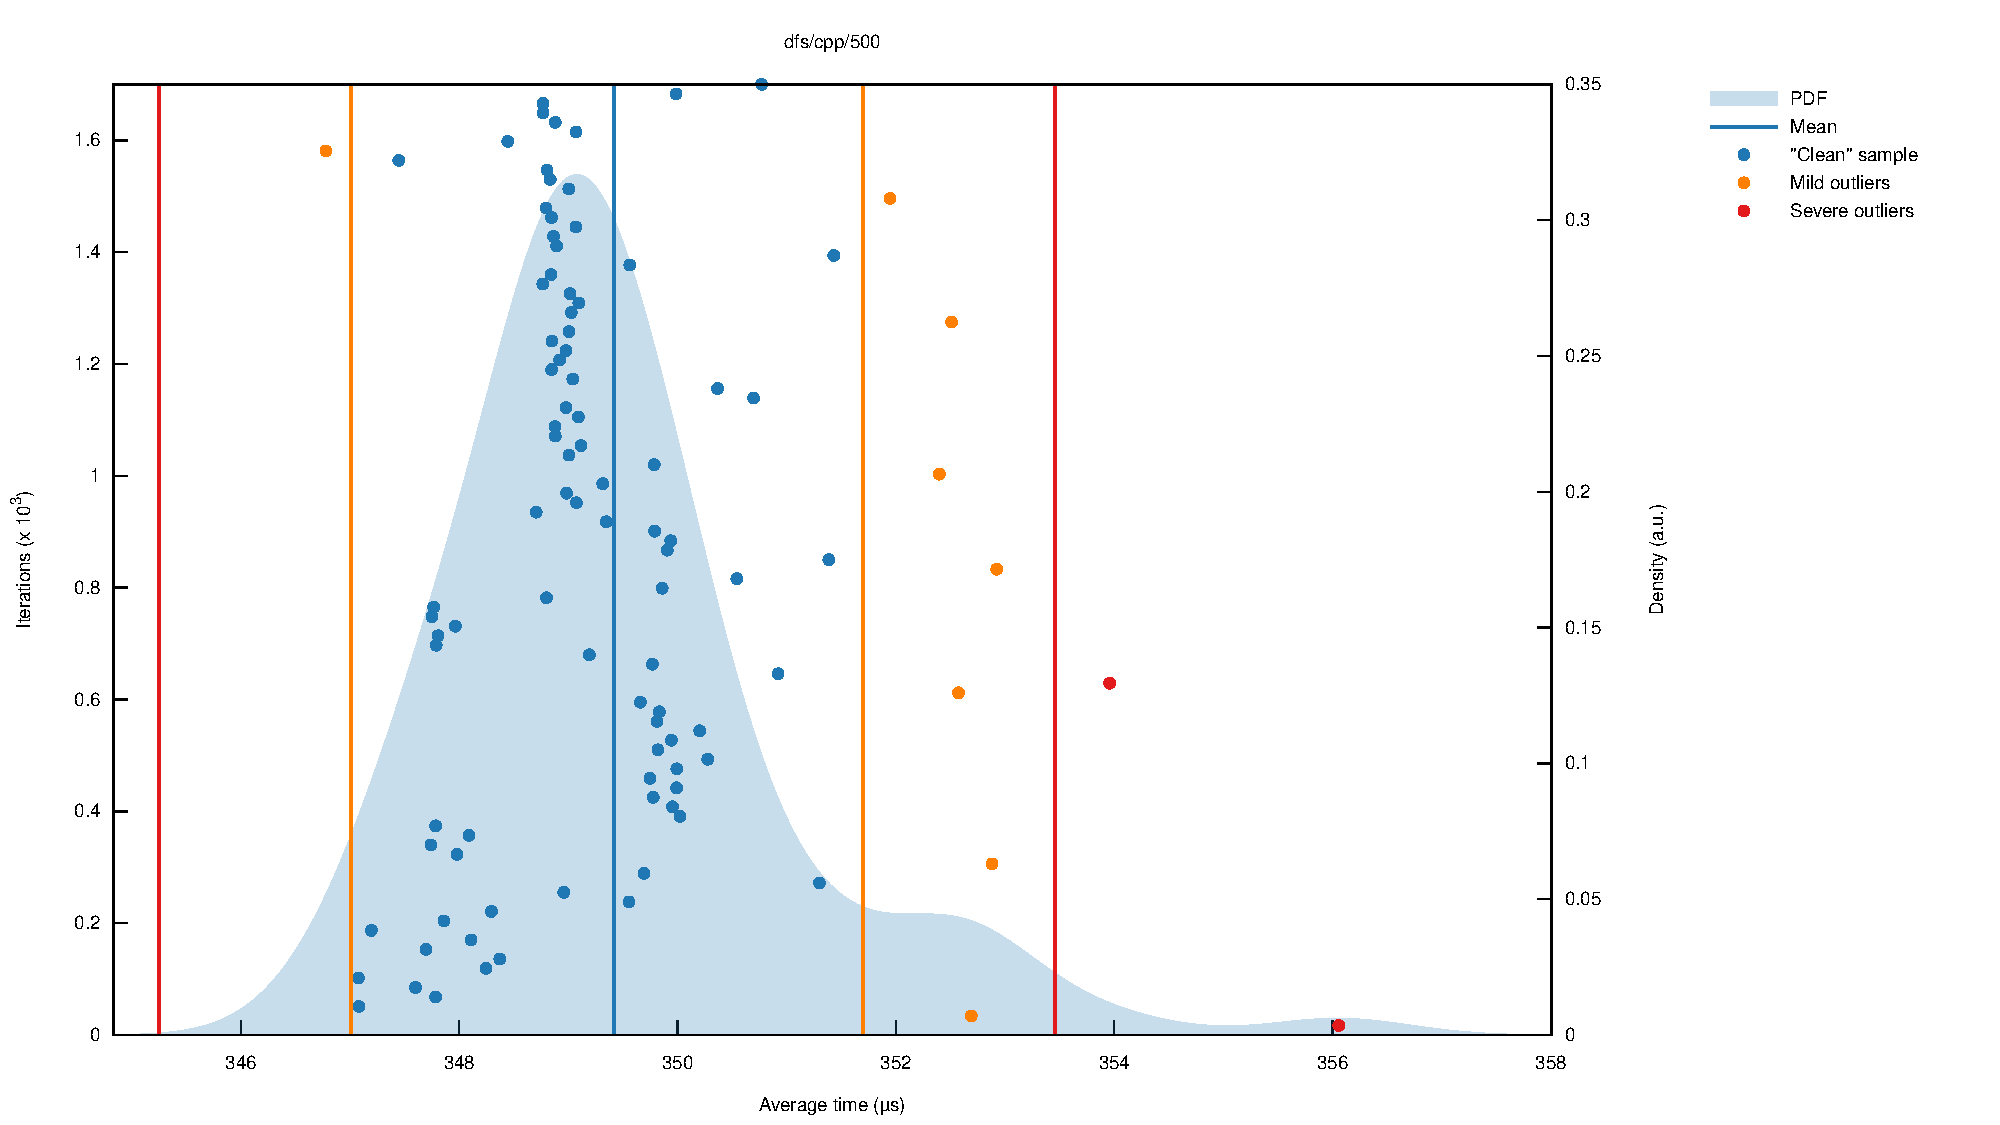
\includegraphics[width=\textwidth]{figures/cpp-dfs-500.pdf}
  \label{graph:cpp-dfs-slope}
\end{figure}
\FloatBarrier

O gráfico da figura~\ref{graph:cpp-dfs-slope} segue as mesmas
especificações do gráfico da figura~\ref{graph:rust-dfs-slope},
discutida anteriormente. Nesse caso, o tempo médio de execução do
algoritmo é aproximadamente 349 ms, sendo 10 vezes mais rápida do que
a versão em Rust, algo que se mantém consistente independente do
tamanho do grafo.

Quanto ao gráfico de regressão das amostras, ele segue o padrão do
teste realizado no código em Rust:

\begin{figure}[!ht]
  \centering
  \caption{Gráfico de regressão das amostras do Micro Benchmark
  estatístico da DFS em C++.}
  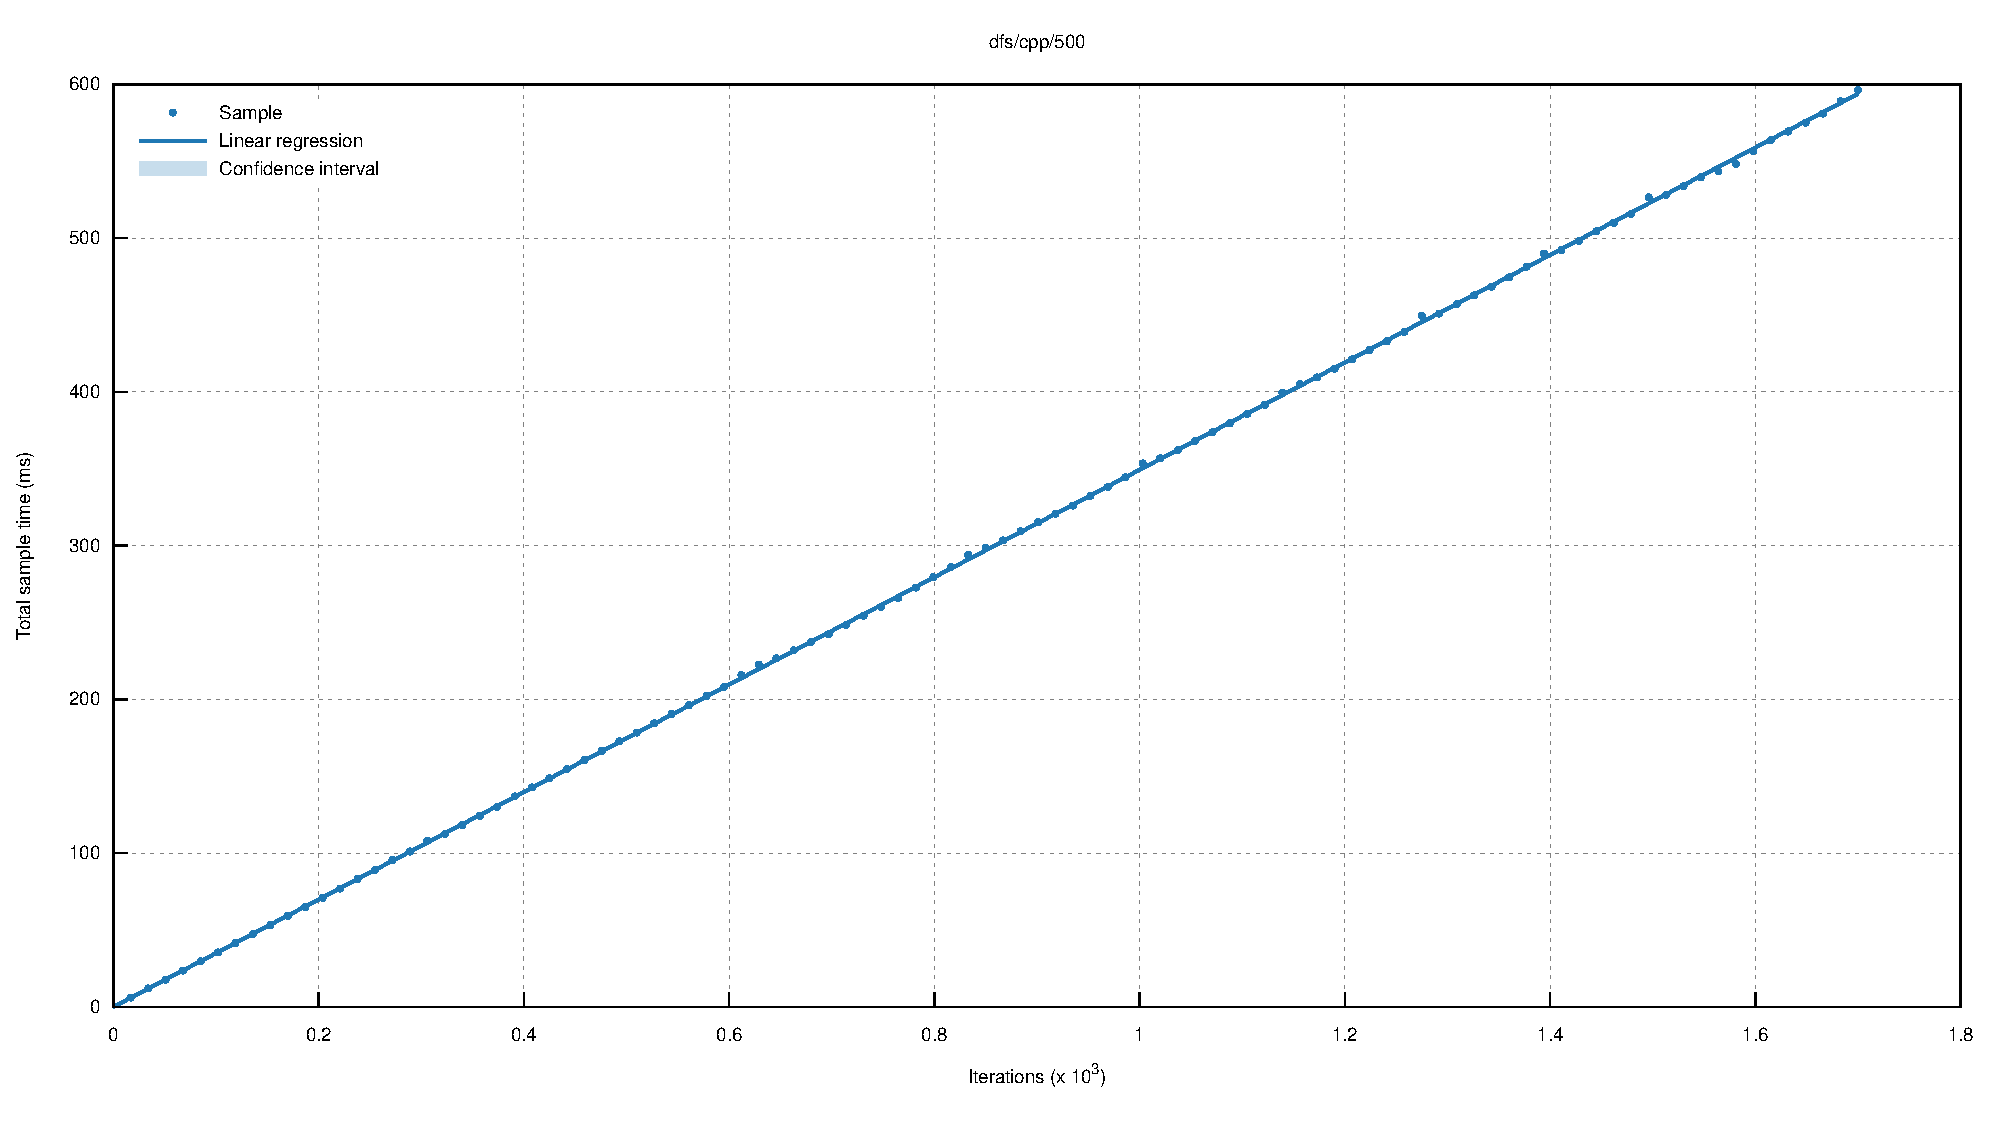
\includegraphics[width=\textwidth]{figures/cpp-dfs-500-regression.pdf}
\end{figure}
\FloatBarrier

\subsubsection{Micro Benchmark de alta precisão}

Nos testes de Micro Benchmarking de alta precisão tivemos os
seguintes resultados:

\begin{table}[!ht]
  \centering
  \caption{Resultados do Micro Benchmark de alta precisão da DFS.}
  \begin{tabular}{llr}
    \toprule
    Métricas                 &  C++    & Iterador em Rust \\
    \midrule
    Quantidade de instruções      & 85926683  & 173801339 \\
    Acertos no Cache L1           & 122803778 & 208565341 \\
    Acertos no Cache LL           & 873133    & 193603    \\
    Acertos na RAM                & 429925    & 441938    \\
    Quantidade de ciclos estimada & 142216818 & 225001186 \\
    \bottomrule
  \end{tabular}
  \label{tab:microhp-dfs}
\end{table}
\FloatBarrier

Em forma de gráfico, tivemos:

\begin{figure}[!ht]
  \centering
  \caption{Gráfico do Micro Benchmark de alta precisão da DFS.}
  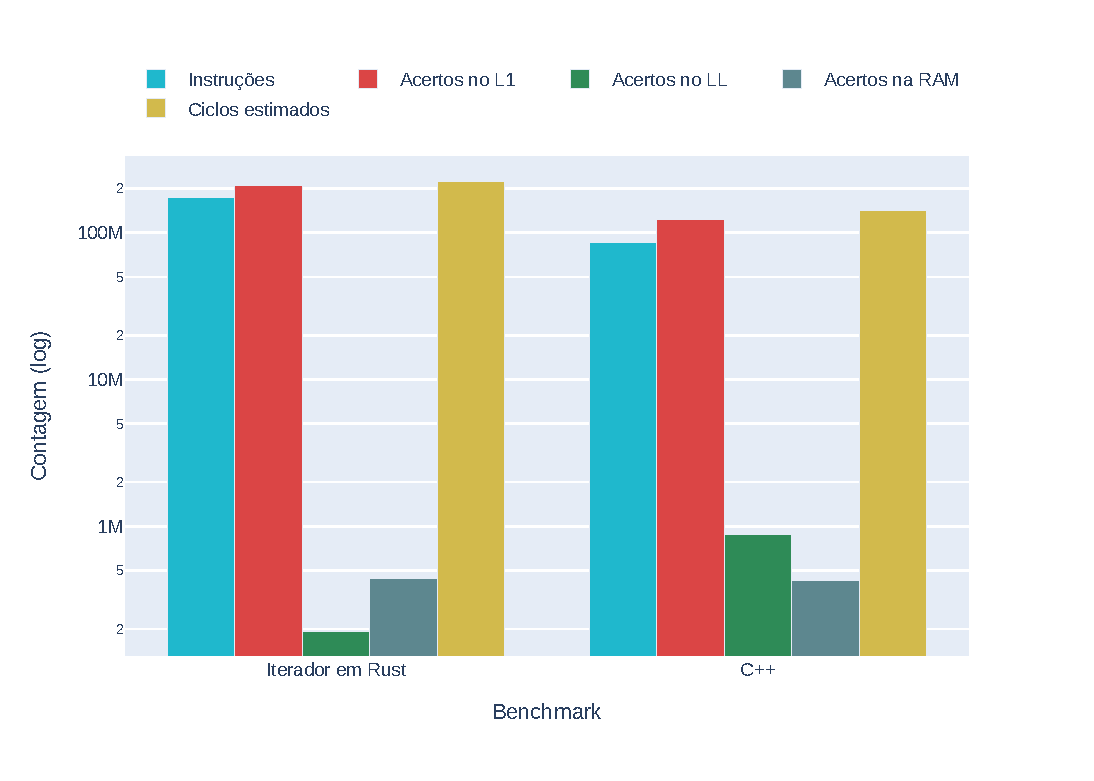
\includegraphics[width=\textwidth]{figures/benchmark-chart.pdf}
\end{figure}
\FloatBarrier

Na tabela~\ref{tab:microhp-dfs} é possível perceber que a versão em
C++ realiza em torno de 2 vezes menos a quantidade de instruções que
a versão em Rust faz. Entretanto também é possível notar que a versão
em Rust usa mais o cache L1, em torno de 1.7 vezes mais, e bem menos
o cache LL em relação a versão em C++, em torno de 4.5 vezes menos,
indicando que o uso de cache é mais otimizado na versão em Rust.
Também é possível notar que a versão em C++ precisa de 1.5 vezes
menos ciclos na CPU para terminar sua computação. Isso significa que,
mesmo aproveitando o cache, a versão da DFS em forma de iteradores em
Rust precisou de mais instruções para completar, o que é razoável
dado a flexibilidade do uso dessa implementação.
